% STEP 1: Choose oneside or twoside. Use the 'draft' option a lot when writing.
\documentclass[english, oneside]{HYgradu}

\usepackage[utf8]{inputenc} % For UTF8 support. Use UTF8 when saving your file.
\usepackage{lmodern} % Font package
\usepackage{textcomp}
\usepackage[pdftex]{color, graphicx} % For pdf output and jpg/png graphics
\usepackage[pdftex, plainpages=false]{hyperref} % For hyperlinks and pdf metadata
\usepackage{fancyhdr} % For nicer page headers
%\usepackage{tikz} % For making vector graphics (hard to learn but powerful)
%\usepackage{wrapfig} % For nice text-wrapping figures (use at own discretion)
\usepackage{amsmath, amssymb} % For better math
%\usepackage[round]{natbib} % For bibliography
\usepackage[footnotesize,bf]{caption} % For more control over figure captions

\fussy % Probably not needed but you never know...

% OPTIONAL STEP: Set up properties and metadata for the pdf file that pdfLaTeX makes.
% But you don't really need to do this unless you want to.
%\hypersetup{
%    bookmarks=true,         % show bookmarks bar first?
%    unicode=true,           % to show non-Latin characters in Acrobat’s bookmarks
%    pdftoolbar=true,        % show Acrobat’s toolbar?
%    pdfmenubar=true,        % show Acrobat’s menu?
%    pdffitwindow=false,     % window fit to page when opened
%    pdfstartview={FitH},    % fits the width of the page to the window
%    pdftitle={},            % title
%    pdfauthor={},           % author
%    pdfsubject={},          % subject of the document
%    pdfcreator={},          % creator of the document
%    pdfproducer={pdfLaTeX}, % producer of the document
%    pdfkeywords={something} {something else}, % list of keywords for
%    pdfnewwindow=true,      % links in new window
%    colorlinks=true,        % false: boxed links; true: colored links
%    linkcolor=black,        % color of internal links
%    citecolor=black,        % color of links to bibliography
%    filecolor=magenta,      % color of file links
%    urlcolor=cyan           % color of external links
%}

% STEP 2:
% Set up all the information for the title page and the abstract form.
% Replace parameters with your information.
\title{Your Title Here}
\author{Anni Järvenpää}
\date{\today}
\level{Master's thesis}
\faculty{Faculty of Science}
\department{Department of Physics}
\address{PL 64 (Gustaf Hällströmin katu 2a)\\00014 University of Helsinki}
\subject{Astronomy}
\prof{Associate Professor Peter Johansson}{Dr. Till Sawala}
\censors{prof. Smith}{doc. Smythe}{}
\depositeplace{}
\additionalinformation{}
\numberofpagesinformation{\numberofpages\ pages}
\classification{}
\keywords{Your keywords here}
\quoting{}%``Bachelor's degrees make pretty good placemats if you get them laminated.'' \\---Jeph Jacques}

\begin{document}

% Generate title page.
\maketitle

% STEP 3:
% Write your abstract (of course you really do this last).
% You can make several abstract pages (if you want it in different languages),
% but you should also then redefine some of the above parameters in the proper
% language as well, in between the abstract definitions.
\begin{abstract}
Abstract goes here.
\end{abstract}

% Place ToC
\mytableofcontents



% -----------------------------------------------------------------------------------
% STEP 4: Write the thesis.
% Your actual text starts here. You shouldn't mess with the code above the line except
% to change the parameters. Removing the abstract and ToC commands will mess up stuff.
\chapter{Introduction}

\section{TL;DR version of prerequisite information}
\begin{enumerate}
	\item galaxies form
	\begin{itemize}
		\item Why?
		\item When?
		\item How?
		\item Where?
	\end{itemize}
	\item galaxies form in groups
	\item our local group is one of these
	\item something about large scale distribution of galaxies
\end{enumerate}

\section{History of Local Group Research}
LG objects visible with naked eye -> realization they are something outside our galaxy -> realization they are something very much like our galaxy

First determining distance was difficult, now mass is more interesting question

\section{Aim of This Thesis}
Whatever the main results end up being, presented in somewhat coherent manner and hopefully sugar-coated enough to sound Important and Exciting.


\chapter{Theoretical Background}
Think whether LG or LCDM first
%theorythingies from Fattahi paper introduction
\section{Local Group}
Definition of galaxy group, our local group is one of these.

Mass estimate (Li, Yang masses for the LG and MW)

Maybe something about scale of things in our universe, what are galaxy groups made of, what do you get if you go one distance scale up, what's different in galaxy clusters
\subsection{Structure}
Galaxies that are part of LG, distribution of smaller ones around bigger ones

Current mass estimates (at least timing argument, hubble flow and maybe satellites)

\subsection{Evolution}
How have we ended up in a situation described earlier? What will happen in future?


\section{Expanding universe}
\subsection{Discovery}
Make maths, add cosmological constant, make observations, remove cosmological constant

Enough cosmology here or in other sections to make other parts of thesis to make sense and to suffice as master's thesis. How much is enough for the latter?

\subsection{$\Lambda$CDM Cosmology}


\subsection{Hubble flow}
What is, where seen, what means, how to measure, hotness/coldness

Plot: observations with fitted hubble flow


\section{Mathematical and statistical methods}
\subsection{Regression Analysis}
line fitting and other trivial things

\subsection{Statistical testing}
ks-test, maybe others if used, background info about distributions etc in general

\section{Cluster Analysis}
DBSCAN

\chapter{general simulation thingies}
Data used here from EAGLE which uses modified GADGET-2 which is a tree-code that uses leapfrog, other integrators also briefly introduced?
\section{N-body simulations}
\subsection{Hierarchical Tree Algorithm}
\subsection{Numerical Integrators}
\subsection{Halo Finding with Subfind} %iannuzzi thesis
%merger tree mentioned in todo, is it relevant?

\section{Description of actual simulations used}
Volume, number of particles, compare to other simulations, where better and where maybe worse

Resimulation of interesting regions

Simulation has same parameters as EAGLE
800 Mpc volume used
schaye 2015 paper
DM-only parts: Volker-Springer Gadget and Gadget 2 papers 1999 and 2005 or something,     gravity part is more interesting than SPH 
Zooms can use multiple meshes, only one is used here
gravitational softening

\chapter{Findings from DMO Halo Catalogue Analysis}
\section{Selection of Local Group analogues}
criteria, how many found, what are like (some plots maybe? distributions of masses, separations, velocities or correlations between two of those?). This might be part of previous chapter too (relevant to resimulation)?

\section{Local Anisotropy of the Hubble Flow}
Hopefully there's something at least mildly interesting to report when I get to look at the new data

%\subsection{Hubble Flow Fitting}

\begin{figure}
   \centering
   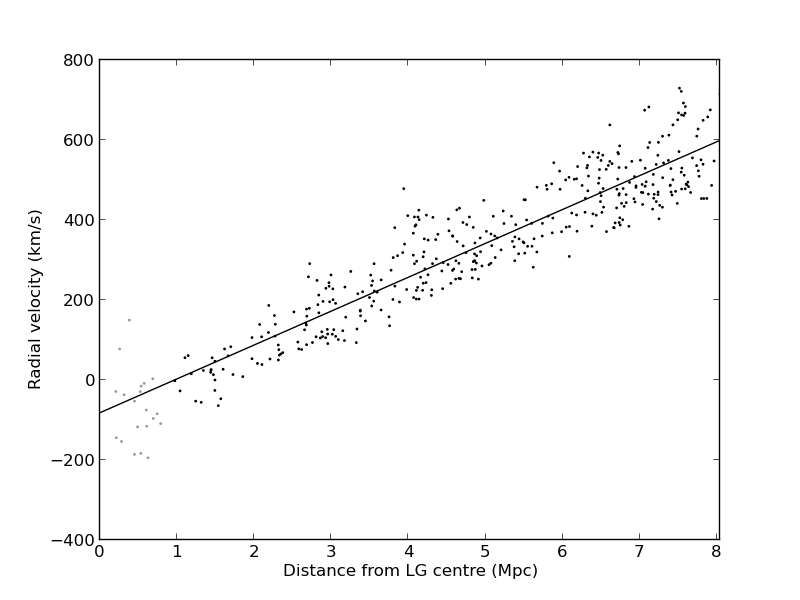
\includegraphics[width=\textwidth]{kuvat/hubbleflow.png}
   \caption{Radial velocities of haloes as a function of distance. Best fit to Hubble flow shown with solid line. Nearby points ignored when fitting shown in gray.}\label{fig:hubbleflow}
\end{figure}

\begin{figure}
   \centering
   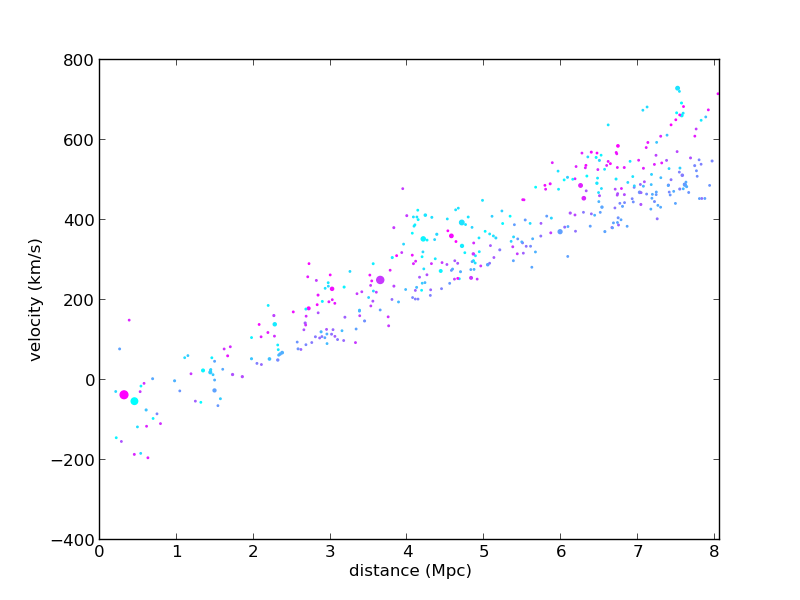
\includegraphics[width=\textwidth]{kuvat/hubbleflow-colour.png}
   \caption{Hubble flow with colours depicting angular disstance from line connecting Milky Way and Andromeda counterparts in simulation.}\label{fig:hubbleflow-colour}
\end{figure}

\begin{figure}
   \centering
   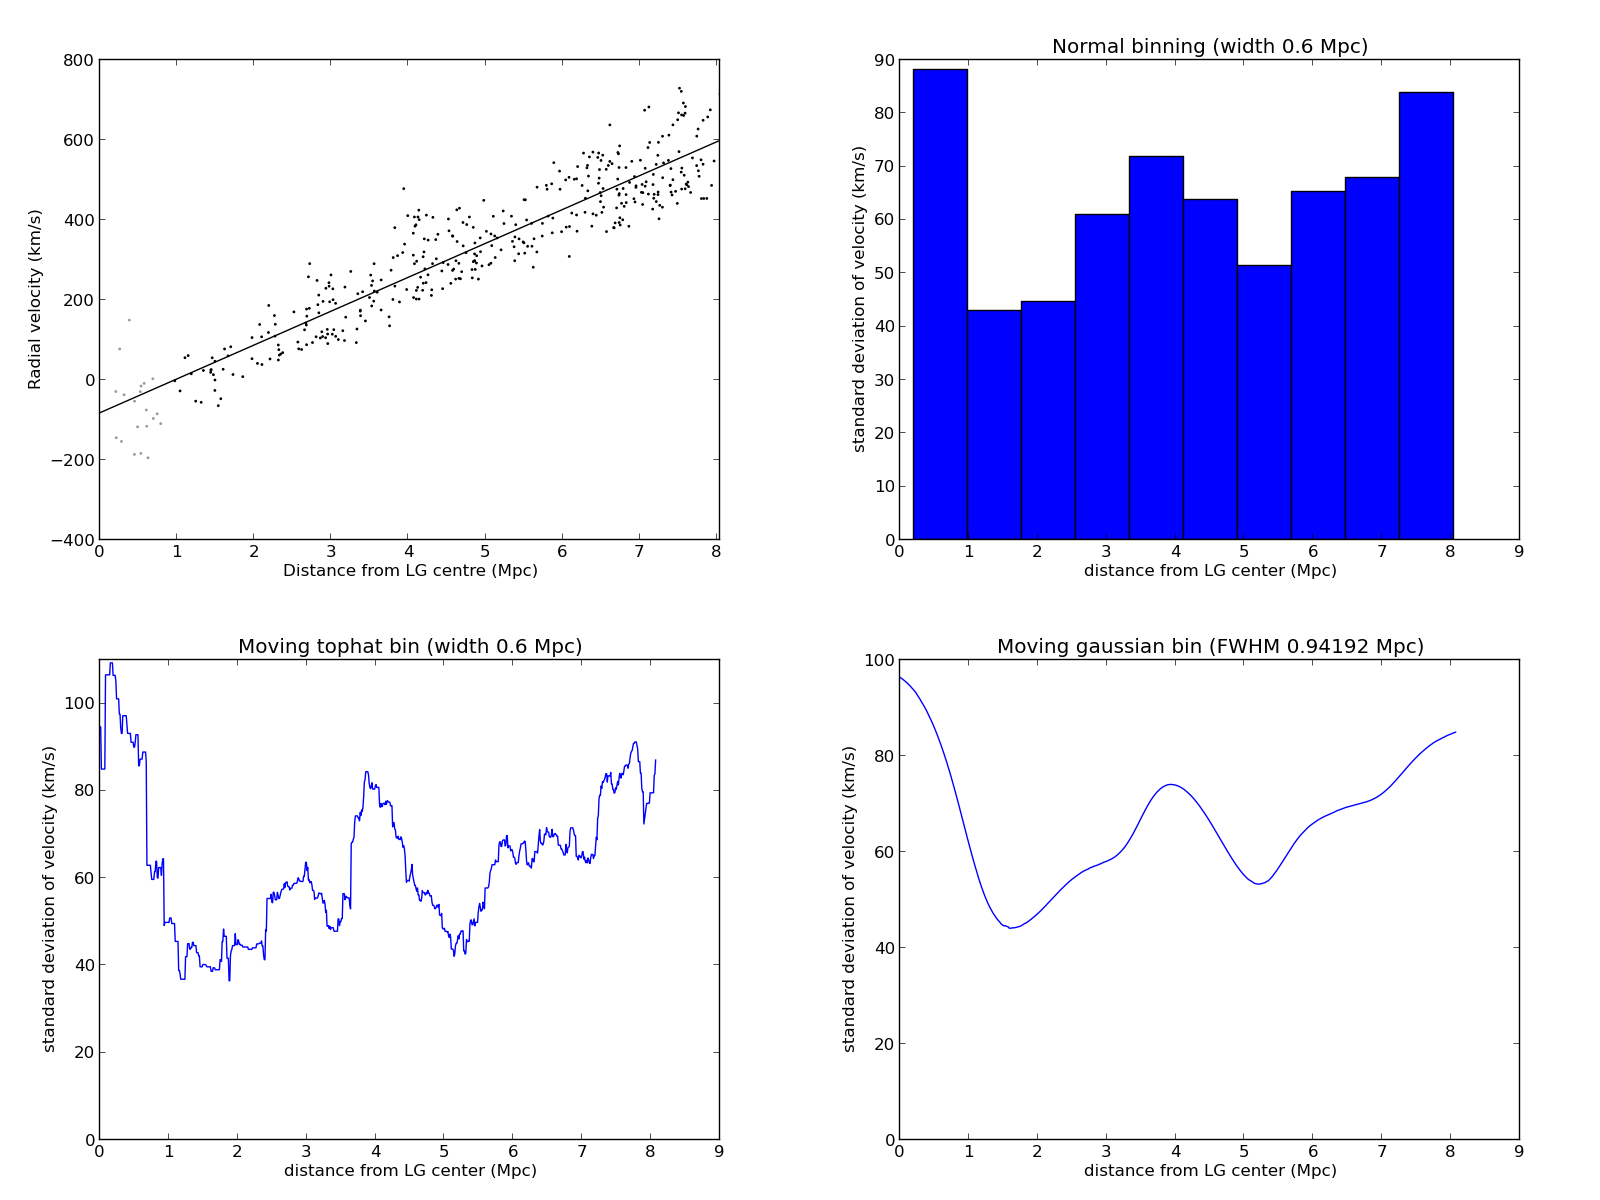
\includegraphics[width=\textwidth]{kuvat/velocitydispersion.png}
   \caption{Velocity dispersion of Hubble flow.}\label{fig:velocitydispersion}
\end{figure}

\begin{figure}
   \centering
   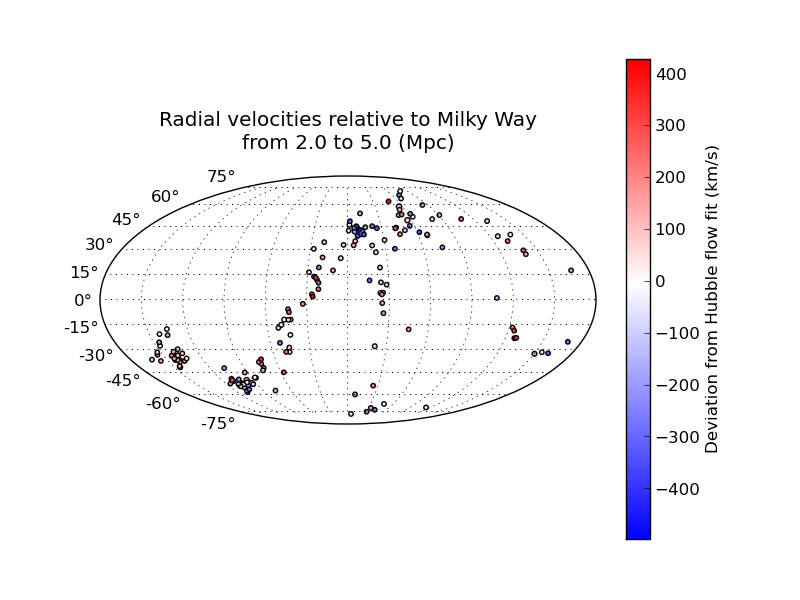
\includegraphics[width=\textwidth]{kuvat/anisotropy-aligned.png}
   \caption{Haloes with distances between 2 and 5 Mpc as seen from Mily Way counterpart in simulation. Colours depict deviations from best linear Hubble flow fit ignoring haloes up to 2 Mpc away, blue end meaning haloes coming closer faster than expected and redder colours moving away.}\label{fig:anisotropymap}
\end{figure}

\begin{figure}
   \centering
   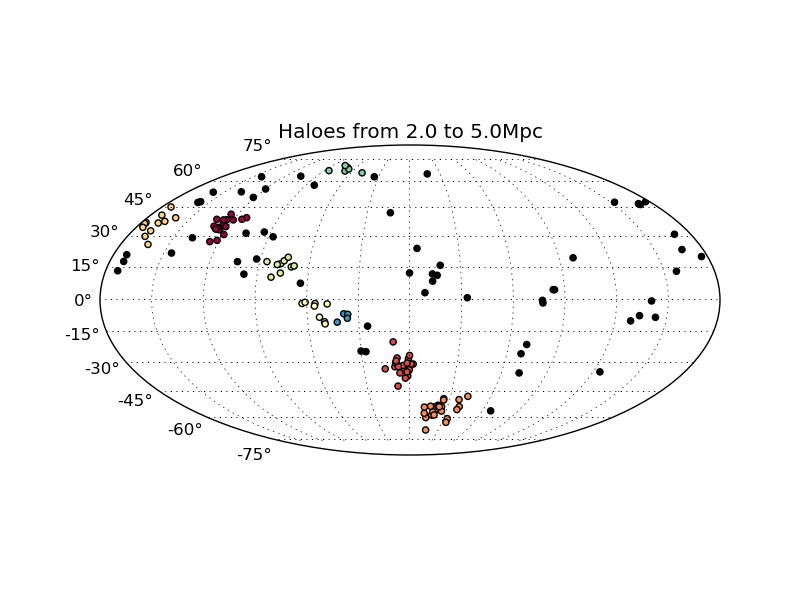
\includegraphics[width=\textwidth]{kuvat/clustering-ms5eps2.png}
   \caption{Dark matter haloes with distances from 2 to 5 Mpc grouped to clusters using DBSCAN clustering algorithm. Parameters used for this plot were ms=5 and eps=2.}\label{fig:clustering}
\end{figure}

\begin{figure}
   \centering
   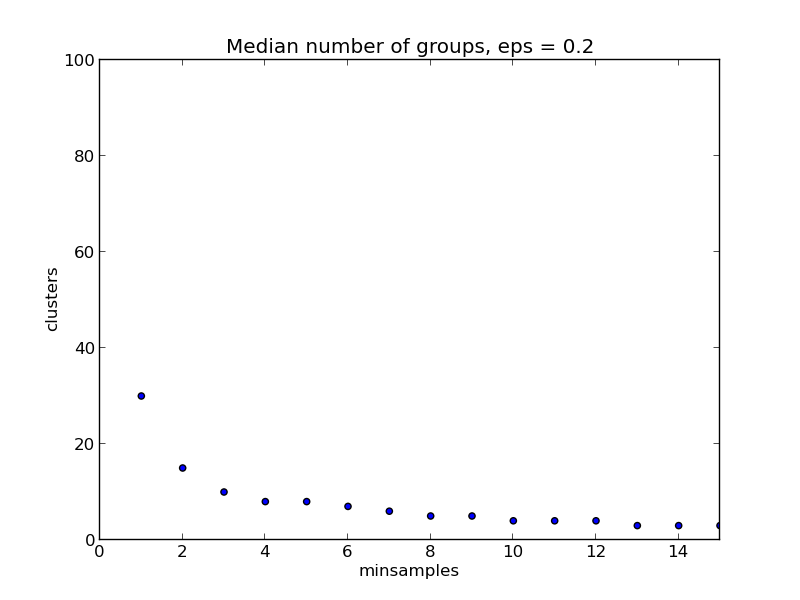
\includegraphics[width=\textwidth]{kuvat/eps-02.png}
   \caption{Median number of clusters found with constant eps on different minsamples.}\label{fig:epseffect}
\end{figure}

\begin{figure}
   \centering
   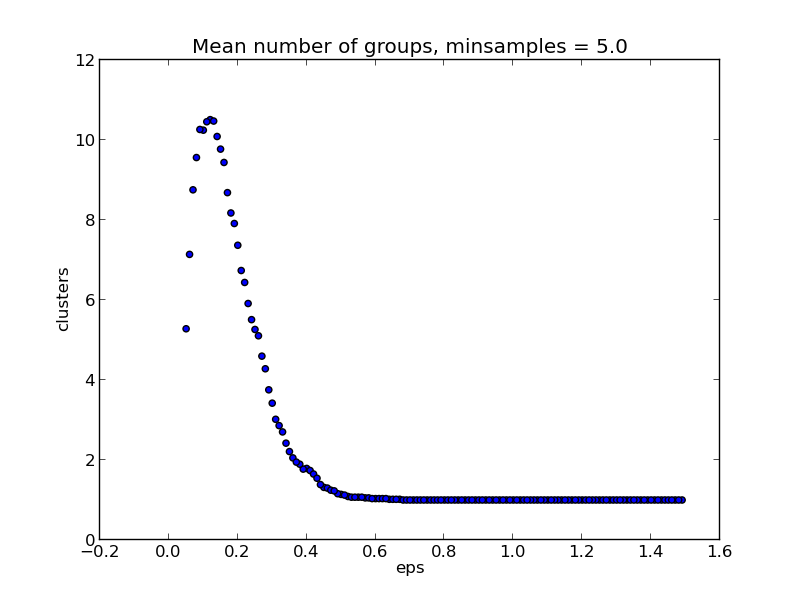
\includegraphics[width=\textwidth]{kuvat/ms-5.png}
   \caption{Mean number of clusters found with constant ms on different eps.}\label{fig:mseffect}
\end{figure}

\begin{figure}
   \centering
   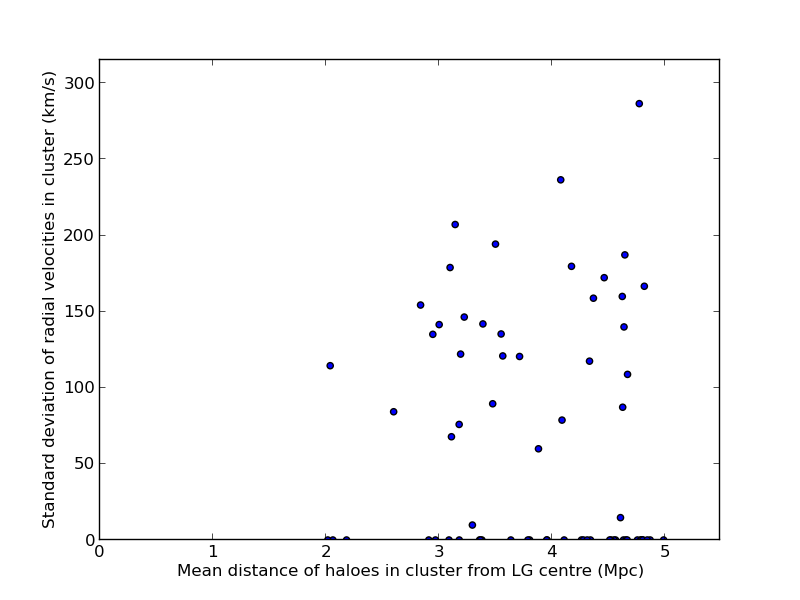
\includegraphics[width=\textwidth]{kuvat/diststd-113.png}
   \caption{Standard deviation of velocities within cluster as a function of distance.}\label{fig:diststd}
\end{figure}

\section{Statistical Estimate of the Local Group Mass}
Analysis similar to Fattahi et al 2016 paper

%\chapter{SIBELIUS project}
% Simulations Beyond the Local Universe
%
%\section{Hubble Flow Fitting}
%
% %if results
%\chapter{Conclusions}

\chapter{Conclusions}





% STEP 5:
% Uncomment the following lines and set your .bib file and desired bibliography style
% to make a bibliography with BibTeX.
% Alternatively you can use the thebibliography environment if you want to add all
% references by hand.

%\clearpage
%\addcontentsline{toc}{chapter}{Bibliography} % This lines adds the bibliography to the ToC
%\bibliographystyle{plain}
%\bibliography{foo.bib}


\end{document}

